\documentclass[crop,tikz]{standalone}
\usetikzlibrary{decorations.pathmorphing,positioning}

\begin{document}
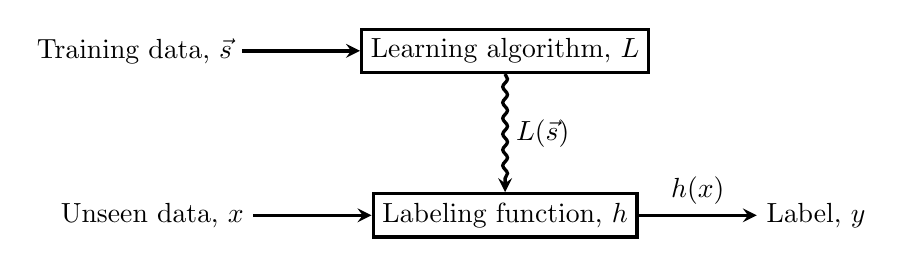
\begin{tikzpicture}[node distance=1.5cm]
  \node[rectangle,very thick,draw] (learning) {Learning algorithm, $L$};
  \node[rectangle,very thick,draw,below=of learning] (labeling) {Labeling function, $h$};
  \node[left=of learning] (train) {Training data, $\vec{s}$};
  \node[left=of labeling] (unseen) {Unseen data, $x$};
  \node[right=of labeling] (label) {Label, $y$};

  \draw[-stealth,very thick] (train) -- (learning);
  \draw[-stealth,very thick] (unseen) -- (labeling);
  \draw[-stealth,very thick] (labeling) -- node[above] {$h(x)$} (label);
  \draw[-stealth,very thick,decorate,
    decoration={snake,segment length=2mm,amplitude=.3mm,post length=1.5mm}]
    (learning) -- node[right] {$L(\vec{s})$} (labeling);
\end{tikzpicture}
\end{document}
